\chapter{Wirtinger Flow}

The whole thing about \emph{Wirtinger Flow} variants started with the seminal work of Candes and Soltanolkotabi\cite{bib:wf}.
The most important improvements chronologically were done by Candes and Chen\cite{bib:twf}, Kolte and Özgür\cite{bib:itwf}, and Zhang et al.\cite{bib:rfw-irwf}.
For a quite extensive survey on \emph{Wirtinger Flow} variants please refer to Liu et al.\cite{bib:wf-survey}. Chandra et al.\cite{bib:phasepack} 
gathered quite number of \emph{Phase Retrieval} methods including a couple of \emph{Wirtinger Flow} variants in the MATLAB\textregistered\space 
problem solving environment in a uniform manner.\\
We quickly go over the problem formulation, difficulties, algorithms, and at the of the chapter we give some numerical experiments we are going
to refer to in the subsequent chapters.

\section{Problem Formulation}
Consider the ray $\boldsymbol{x} \in \mathbb{C}^{n \times 1}$ is emitted onto the object of interest and the diffracted rays are measured as 
$\boldsymbol{y} \in \mathbb{R}^{m \times 1}$ and is connected to the original ray by $\boldsymbol{y} = \varphi(\boldsymbol{A}\boldsymbol{x})$,
where $\boldsymbol{A} \in \mathbb{C}^{m \times n}$ and $\varphi$ the usual element-wise absolute value(or the squared absolute value) from 
$\mathbb{C}^{m \times 1}$ to $\mathbb{R}^{m \times 1}$.\\
Candes and Soltanolkotabi\cite{bib:wf} considered $\varphi$ to be squared element-wise absolute value and the loss function to be quadratic. 
The summary for all the variants in terms of formulation is in table\ref{tab:formulation}  


\begin{table}
	\centering
	\begin{tabular}{||c l c||} 
	 \hline
	 \emph{Wirtinger Flow} Variant 			& $\varphi$ 						& loss functions\\ [0.5ex] 
	 \hline\hline
	 Wirtinger Flow 			 			& $\left|\boldsymbol{z}\right|^2$ 	& quadratic 	\\ 
	 Truncated Wirtinger Flow   			& $\left|\boldsymbol{z}\right|^2$ 	& quadratic 	\\
	 Incrementally Truncated Wirtinger Flow & $\left|\boldsymbol{z}\right|^2$  	& quadratic 	\\
	 Reshaped Wirtinger Flow 				& $\left|\boldsymbol{z}\right|$ 	& quadratic 	\\
	 Incrementally Reshaped Flow 			& $\left|\boldsymbol{z}\right|$ 	& quadratic 	\\ [1ex] 
	 \hline
	\end{tabular}
	\caption{$\varphi$ and the loss function used in \cite{bib:wf}, \cite{bib:twf}, \cite{bib:itwf}, \cite{bib:rfw-irwf}}
	\label{tab:formulation}
	\end{table}
\section{Difficulties}

The loss function is non-convex. Set $n=1$, $m=2$, $\boldsymbol{x}_1 = \begin{pmatrix}1+i\end{pmatrix}^{1 \times 1}$, 
$\boldsymbol{x}_2 = \begin{pmatrix}-1-i\end{pmatrix}^{1 \times 1}$, $\boldsymbol{A}=\begin{pmatrix}1\\i \end{pmatrix}^{2 \times 1}$, 
$\boldsymbol{y}=\begin{pmatrix}1\\2 \end{pmatrix}^{2 \times 1}$, and $\lambda=1/2$ to build a counterexample. Non-convexity is bad news for 
optimization as it can be seen vividly in \cite{bib:opt-boyd} and \cite{bib:opt-wright}. To make the matter worse the loss function is not 
holomorphic( it can be easily seen that Cauchy-Riemann equations\cite{bib:complex-ahl} do not hold) and therefore complex differentiability 
is out of the question\cite{bib:complex-ahl}.   


% \begin{equation} \label{prob:mainproblem}
% 	Recover $\boldsymbol{x} \in \mathbb{R}^n/\mathbb{C}^n$ from measurements $y_i$ given by
% 	\begin{flalign}
% 		y_i=\left|\langle \boldsymbol{a}_i,\mathbf{x}\rangle\right|, \quad \text{for }\; i=1,\cdots,m, \label{eq:mainproblem}
% 	\end{flalign}
% 	where $\boldsymbol{a}_i \in \mathbb{R}^n/\mathbb{C}^n$ are random design vectors (known). 
% \end{equation}









% This file was created with tikzplotlib v0.10.1.
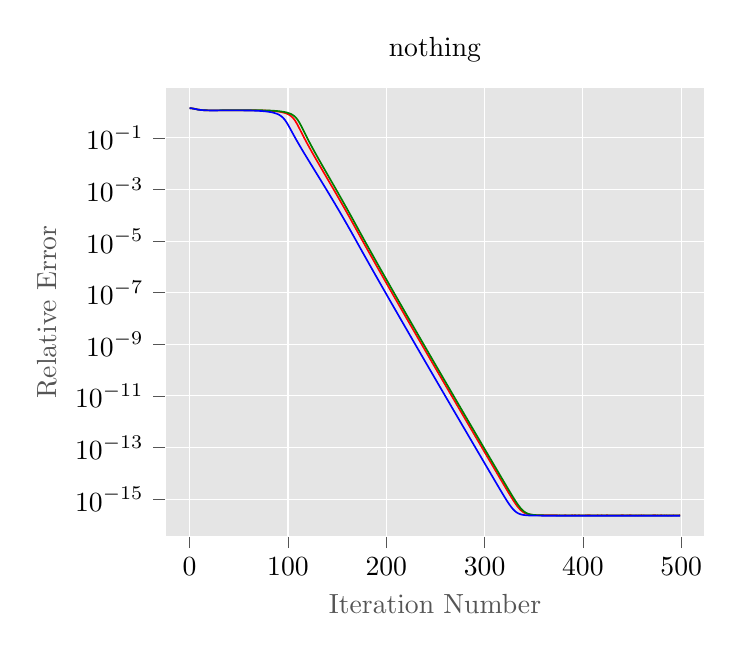
\begin{tikzpicture}

    \definecolor{dimgray85}{RGB}{85,85,85}
    \definecolor{gainsboro229}{RGB}{229,229,229}
    \definecolor{green01270}{RGB}{0,127,0}
    
    \begin{axis}[
    axis background/.style={fill=gainsboro229},
    axis line style={white},
    log basis y={10},
    tick align=outside,
    tick pos=left,
    title={nothing},
    x grid style={white},
    xlabel=\textcolor{dimgray85}{Iteration Number},
    xmajorgrids,
    xmin=-24.95, xmax=523.95,
    xtick style={color=dimgray85},
    y grid style={white},
    ylabel=\textcolor{dimgray85}{Relative Error},
    ymajorgrids,
    ymin=3.6493401978314e-17, ymax=8.71028284657391,
    ymode=log,
    ytick style={color=dimgray85},
    ytick={1e-19,1e-17,1e-15,1e-13,1e-11,1e-09,1e-07,1e-05,0.001,0.1,10,1000},
    yticklabels={
      \(\displaystyle {10^{-19}}\),
      \(\displaystyle {10^{-17}}\),
      \(\displaystyle {10^{-15}}\),
      \(\displaystyle {10^{-13}}\),
      \(\displaystyle {10^{-11}}\),
      \(\displaystyle {10^{-9}}\),
      \(\displaystyle {10^{-7}}\),
      \(\displaystyle {10^{-5}}\),
      \(\displaystyle {10^{-3}}\),
      \(\displaystyle {10^{-1}}\),
      \(\displaystyle {10^{1}}\),
      \(\displaystyle {10^{3}}\)
    }
    ]
    \addplot [semithick, red]
    table {%
    0 1.41146316138425
    1 1.41146316138425
    2 1.40289925947244
    3 1.38679784124659
    4 1.36529978433437
    5 1.34097803002281
    6 1.31615135706901
    7 1.29249751852802
    8 1.27099970304206
    9 1.25208715909011
    10 1.23582451949119
    11 1.22207137608901
    12 1.210591278498
    13 1.20111678311499
    14 1.19338407338758
    15 1.18714899824913
    16 1.18219275323113
    17 1.17832229370766
    18 1.1753684081857
    19 1.17318303553412
    20 1.17163661901323
    21 1.1706158386216
    22 1.17002181152124
    23 1.16976871517254
    24 1.16978272314798
    25 1.1700011241142
    26 1.17037150513229
    27 1.17085091021507
    28 1.17140492421237
    29 1.17200667157589
    30 1.17263575202503
    31 1.1732771559605
    32 1.17392021028902
    33 1.17455760173263
    34 1.17518451325278
    35 1.17579789413038
    36 1.17639586924221
    37 1.17697728074084
    38 1.17754134692174
    39 1.17808741865395
    40 1.17861481271637
    41 1.17912270273378
    42 1.17961005113779
    43 1.18007556884873
    44 1.18051769259558
    45 1.18093457261704
    46 1.18132406577057
    47 1.18168373080251
    48 1.18201082376608
    49 1.18230229241008
    50 1.18255476889873
    51 1.18276456055071
    52 1.18292763847137
    53 1.18303962404762
    54 1.18309577331474
    55 1.18309095921073
    56 1.1830196517208
    57 1.1828758958894
    58 1.18265328764438
    59 1.18234494733853
    60 1.18194349086836
    61 1.18144099817821
    62 1.18082897889781
    63 1.18009833479258
    64 1.17923931862534
    65 1.17824148893411
    66 1.17709366011965
    67 1.1757838471044
    68 1.17429920366796
    69 1.17262595337566
    70 1.17074931179087
    71 1.16865339838879
    72 1.16632113625965
    73 1.16373413728985
    74 1.16087257002575
    75 1.15771500683735
    76 1.15423824628681
    77 1.150417105741
    78 1.1462241782151
    79 1.14162954615414
    80 1.13660044329948
    81 1.13110085388634
    82 1.12509103610005
    83 1.11852695389721
    84 1.11135959787467
    85 1.10353417174759
    86 1.09498911609484
    87 1.08565493531728
    88 1.07545278732146
    89 1.06429278862706
    90 1.05207198121076
    91 1.03867190314381
    92 1.02395570626626
    93 1.00776477697677
    94 0.989914852015906
    95 0.970191700051546
    96 0.948346597089692
    97 0.924092118776841
    98 0.897099302227896
    99 0.86699814049022
    100 0.833384857646062
    101 0.795841651124099
    102 0.753977519757002
    103 0.707501532393521
    104 0.656339535168611
    105 0.600795441901377
    106 0.541729547885406
    107 0.480675638795114
    108 0.419772936343581
    109 0.361421632171142
    110 0.307738737295067
    111 0.26008693924877
    112 0.218932208630245
    113 0.184030640531528
    114 0.154740959421387
    115 0.130283356110482
    116 0.10989121534696
    117 0.0928788720244066
    118 0.0786614635176984
    119 0.0667521643384321
    120 0.0567506473342828
    121 0.0483294242029025
    122 0.0412209098496065
    123 0.0352062124639679
    124 0.0301058257289256
    125 0.0257720674382606
    126 0.0220830034073597
    127 0.0189375876564976
    128 0.0162517790915347
    129 0.0139554343421798
    130 0.011989814812972
    131 0.0103055793342805
    132 0.00886116120828561
    133 0.0076214503417456
    134 0.00655671837726513
    135 0.0056417381631742
    136 0.00485505933293749
    137 0.0041784098590951
    138 0.00359619973319607
    139 0.00309510781645162
    140 0.00266373672645189
    141 0.00229232361946047
    142 0.00197249708397916
    143 0.00169707222355843
    144 0.00145987748546232
    145 0.00125560797126731
    146 0.00107970091069659
    147 0.000928229740995337
    148 0.000797813849632033
    149 0.000685541538112704
    150 0.000588904172641009
    151 0.000505739821586514
    152 0.00043418495465638
    153 0.000372633005690417
    154 0.000319698789150546
    155 0.000274187916851368
    156 0.000235070492039117
    157 0.000201458467201694
    158 0.000172586143719474
    159 0.000147793368673835
    160 0.000126511049282291
    161 0.000108248660539703
    162 9.25834683647198e-05
    163 7.91512302394395e-05
    164 6.7638169110112e-05
    165 5.77740451183679e-05
    166 4.93261743296969e-05
    167 4.20942646636626e-05
    168 3.59059572487204e-05
    169 3.06129768761526e-05
    170 2.60965753543401e-05
    171 2.22531532706819e-05
    172 1.89812454311544e-05
    173 1.61948983776001e-05
    174 1.38212599124961e-05
    175 1.17985504513911e-05
    176 1.00743543554154e-05
    177 8.60417967543263e-06
    178 7.35024325933872e-06
    179 6.28044524570788e-06
    180 5.3675028447598e-06
    181 4.58821819946388e-06
    182 3.92285919555838e-06
    183 3.35463548984037e-06
    184 2.86925486604286e-06
    185 2.45454740209878e-06
    186 2.10014691985281e-06
    187 1.79722085310816e-06
    188 1.5382410659164e-06
    189 1.316789324682e-06
    190 1.12739211182864e-06
    191 9.65380296207781e-07
    192 8.26769871560314e-07
    193 7.08160560492756e-07
    194 6.06649575329092e-07
    195 5.19758243626485e-07
    196 4.45369557540018e-07
    197 3.81675002854851e-07
    198 3.27129274158127e-07
    199 2.80411694458072e-07
    200 2.40393336756357e-07
    201 2.06108996713744e-07
    202 1.76733293941848e-07
    203 1.51560288226998e-07
    204 1.29986089168152e-07
    205 1.11494015891291e-07
    206 9.56419297998126e-08
    207 8.20514196180194e-08
    208 7.03985657594616e-08
    209 6.04060516438381e-08
    210 5.18364240784243e-08
    211 4.44863341383538e-08
    212 3.81816149142787e-08
    213 3.27730736981484e-08
    214 2.8132894241809e-08
    215 2.41515600663125e-08
    216 2.07352229003362e-08
    217 1.78034514585363e-08
    218 1.52873052705742e-08
    219 1.31276863606143e-08
    220 1.1273928473837e-08
    221 9.68258943922212e-09
    222 8.31641725767732e-09
    223 7.14346480515667e-09
    224 6.1363316776631e-09
    225 5.27151483466775e-09
    226 4.52885235072693e-09
    227 3.89104686903283e-09
    228 3.34325728109043e-09
    229 2.87274882595028e-09
    230 2.46859321390618e-09
    231 2.12141159208716e-09
    232 1.82315421114994e-09
    233 1.5669115253716e-09
    234 1.34675223221094e-09
    235 1.15758438914256e-09
    236 9.95036308934939e-10
    237 8.55354411983437e-10
    238 7.35315601263725e-10
    239 6.3215210395592e-10
    240 5.43486986065499e-10
    241 4.67278826678436e-10
    242 4.01774248332127e-10
    243 3.45467176517559e-10
    244 2.9706388027944e-10
    245 2.5545296729459e-10
    246 2.19679626880223e-10
    247 1.88923522544413e-10
    248 1.62479812678087e-10
    249 1.39742857165126e-10
    250 1.20192225629681e-10
    251 1.03380686260031e-10
    252 8.89238896542633e-11
    253 7.64915105086944e-11
    254 6.57996392170124e-11
    255 5.66042489574818e-11
    256 4.86955805223458e-11
    257 4.18933251160877e-11
    258 3.60424782313485e-11
    259 3.10097860979146e-11
    260 2.66806855478014e-11
    261 2.29566797021466e-11
    262 1.97530801819149e-11
    263 1.69970688862008e-11
    264 1.46260317164814e-11
    265 1.25861256591584e-11
    266 1.08310480998092e-11
    267 9.3209807059791e-12
    268 8.02167803975227e-12
    269 6.90368841562144e-12
    270 5.94168076590352e-12
    271 5.1138668899684e-12
    272 4.40150665893592e-12
    273 3.78847967988878e-12
    274 3.26091908952998e-12
    275 2.80689700507714e-12
    276 2.41615131644146e-12
    277 2.07985396036766e-12
    278 1.79040971416037e-12
    279 1.54128428422886e-12
    280 1.32685585996962e-12
    281 1.14228690302257e-12
    282 9.83415598108055e-13
    283 8.46660041264727e-13
    284 7.28939038453108e-13
    285 6.27600427102824e-13
    286 5.40362798689363e-13
    287 4.65261291957164e-13
    288 4.00606703738447e-13
    289 3.44944411140821e-13
    290 2.97022500560458e-13
    291 2.55763691924486e-13
    292 2.20240783165405e-13
    293 1.89655373360996e-13
    294 1.63320821076484e-13
    295 1.40645965665742e-13
    296 1.21121685876832e-13
    297 1.04309775413308e-13
    298 8.98333930700092e-14
    299 7.73676488633548e-14
    300 6.66330402880405e-14
    301 5.73887830052003e-14
    302 4.94281095933337e-14
    303 4.25723236136907e-14
    304 3.66688047145526e-14
    305 3.15839439846863e-14
    306 2.72052049385742e-14
    307 2.34335390997116e-14
    308 2.01853852086373e-14
    309 1.73882816541301e-14
    310 1.49787402829135e-14
    311 1.29034807578783e-14
    312 1.11165845651646e-14
    313 9.57735404267913e-15
    314 8.25156406372107e-15
    315 7.10946284729784e-15
    316 6.12623707716984e-15
    317 5.27911834319439e-15
    318 4.54992716721267e-15
    319 3.9218467046501e-15
    320 3.38143482856078e-15
    321 2.9158611673796e-15
    322 2.51524465974011e-15
    323 2.17063121464269e-15
    324 1.87446886869303e-15
    325 1.61999578121989e-15
    326 1.40190486100833e-15
    327 1.21454257321246e-15
    328 1.05439612045951e-15
    329 9.17147856759168e-16
    330 8.00774526404244e-16
    331 7.01943216730213e-16
    332 6.18250457258573e-16
    333 5.48067447951626e-16
    334 4.89333327983537e-16
    335 4.40715837791351e-16
    336 4.00404522614526e-16
    337 3.67439856053168e-16
    338 3.40849939004218e-16
    339 3.18815812539134e-16
    340 3.01542239160321e-16
    341 2.87515924890766e-16
    342 2.76761862194095e-16
    343 2.68293889529308e-16
    344 2.61491888499865e-16
    345 2.56211472540159e-16
    346 2.54354182976011e-16
    347 2.49073313621162e-16
    348 2.46855522500262e-16
    349 2.44608423462102e-16
    350 2.43102717579413e-16
    351 2.41822598127878e-16
    352 2.40799071724778e-16
    353 2.39761024109505e-16
    354 2.39352209644643e-16
    355 2.38733958073188e-16
    356 2.38245808402333e-16
    357 2.37791175978896e-16
    358 2.37390712943325e-16
    359 2.37023843687574e-16
    360 2.3681712648991e-16
    361 2.36743274408629e-16
    362 2.36522322507222e-16
    363 2.36359837719669e-16
    364 2.36314332578573e-16
    365 2.36159909940163e-16
    366 2.38093287154551e-16
    367 2.37723962454412e-16
    368 2.35331814578674e-16
    369 2.35104673512767e-16
    370 2.35194288880141e-16
    371 2.37171417688308e-16
    372 2.34849691964025e-16
    373 2.3512032019603e-16
    374 2.35039207524817e-16
    375 2.34783224710028e-16
    376 2.34948097276413e-16
    377 2.34912884039204e-16
    378 2.34855531304134e-16
    379 2.34315255902777e-16
    380 2.34416011529047e-16
    381 2.34487150905616e-16
    382 2.36707703442513e-16
    383 2.34603130972634e-16
    384 2.34465427956739e-16
    385 2.3439837455247e-16
    386 2.34544921217009e-16
    387 2.34452782405739e-16
    388 2.34232514486804e-16
    389 2.36294518706336e-16
    390 2.34411265011646e-16
    391 2.34502888425202e-16
    392 2.36689483801567e-16
    393 2.34419892688076e-16
    394 2.34324248427554e-16
    395 2.34057552914706e-16
    396 2.36163619416043e-16
    397 2.34044664879283e-16
    398 2.34114857090208e-16
    399 2.34202245447081e-16
    400 2.34046613991891e-16
    401 2.34061385794813e-16
    402 2.33953571319778e-16
    403 2.36047479829532e-16
    404 2.34217193178086e-16
    405 2.36142674590822e-16
    406 2.3614083436547e-16
    407 2.36223739245947e-16
    408 2.34118454213855e-16
    409 2.34152928741188e-16
    410 2.33900310565842e-16
    411 2.34006325122669e-16
    412 2.33952920586301e-16
    413 2.33734720905062e-16
    414 2.33734293177394e-16
    415 2.35729318475023e-16
    416 2.3381552791303e-16
    417 2.33850555852379e-16
    418 2.33656763267132e-16
    419 2.35689054012705e-16
    420 2.33924275156626e-16
    421 2.33602892264249e-16
    422 2.33419615831133e-16
    423 2.33543510655773e-16
    424 2.35668691786182e-16
    425 2.35748592736058e-16
    426 2.33433964863134e-16
    427 2.33731233142613e-16
    428 2.33348739540052e-16
    429 2.33471130444629e-16
    430 2.33239242047647e-16
    431 2.33326119644071e-16
    432 2.33376659090518e-16
    433 2.33448691461721e-16
    434 2.33531360986238e-16
    435 2.33301360214615e-16
    436 2.33730494229341e-16
    437 2.33463411179668e-16
    438 2.33467060429152e-16
    439 2.35630629311099e-16
    440 2.35520161001846e-16
    441 2.35578465213516e-16
    442 2.33304102442136e-16
    443 2.33444759827067e-16
    444 2.33486173877886e-16
    445 2.35506228764715e-16
    446 2.33405552774784e-16
    447 2.35338602246061e-16
    448 2.35351494481499e-16
    449 2.35337599693553e-16
    450 2.33361057348535e-16
    451 2.33120923513527e-16
    452 2.33112835317211e-16
    453 2.33057868821037e-16
    454 2.35182653912048e-16
    455 2.33081264660797e-16
    456 2.3304982912054e-16
    457 2.35016594929159e-16
    458 2.33333206580154e-16
    459 2.35136428718065e-16
    460 2.35042746280729e-16
    461 2.33220399873598e-16
    462 2.35345244033489e-16
    463 2.3319165066078e-16
    464 2.33071240429731e-16
    465 2.33325396116024e-16
    466 2.33111975750637e-16
    467 2.33397337302873e-16
    468 2.33219788352129e-16
    469 2.33190060007158e-16
    470 2.33292812552674e-16
    471 2.35143881177173e-16
    472 2.3525350539502e-16
    473 2.35403702546803e-16
    474 2.35239266438805e-16
    475 2.33208546200863e-16
    476 2.3531710494061e-16
    477 2.33261287437452e-16
    478 2.33231724987668e-16
    479 2.35430014256021e-16
    480 2.35384651035166e-16
    481 2.33342581819885e-16
    482 2.33343078030708e-16
    483 2.35063974449359e-16
    484 2.33200777999907e-16
    485 2.35247928343655e-16
    486 2.32769497009069e-16
    487 2.32863351871848e-16
    488 2.3498124925546e-16
    489 2.33036365501604e-16
    490 2.32941557452417e-16
    491 2.33005189764838e-16
    492 2.35188689429557e-16
    493 2.33238716999975e-16
    494 2.33232317200523e-16
    495 2.33058812927575e-16
    496 2.33145781459391e-16
    497 2.3323906320035e-16
    498 2.35147639795929e-16
    499 2.35008438989637e-16
    };
    \addplot [semithick, green01270]
    table {%
    0 1.41296512935814
    1 1.41296512935814
    2 1.40390343594449
    3 1.38692039305203
    4 1.36437855076799
    5 1.33907611761819
    6 1.31347842345842
    7 1.28931315570307
    8 1.26754525268652
    9 1.24855519604334
    10 1.23235454999101
    11 1.2187578570214
    12 1.20749488254218
    13 1.19827467016604
    14 1.19081783484708
    15 1.18487026305005
    16 1.18020689055306
    17 1.17663070823538
    18 1.17396985265664
    19 1.17207427024621
    20 1.17081266580671
    21 1.17007001435772
    22 1.16974567931462
    23 1.16975205438302
    24 1.17001358636409
    25 1.17046601843289
    26 1.17105570584663
    27 1.17173888935868
    28 1.17248085690001
    29 1.17325497195866
    30 1.17404158882654
    31 1.17482690409619
    32 1.17560180758544
    33 1.17636079503411
    34 1.17710099305989
    35 1.17782132895061
    36 1.17852185875543
    37 1.17920325049764
    38 1.17986640723253
    39 1.1805122076625
    40 1.18114133954565
    41 1.18175420205009
    42 1.18235085622646
    43 1.18293100675534
    44 1.18349400222831
    45 1.1840388449127
    46 1.18456420397464
    47 1.1850684284342
    48 1.18554955776038
    49 1.18600532910164
    50 1.18643318082233
    51 1.18683025239747
    52 1.18719338090797
    53 1.18751909444749
    54 1.18780360275345
    55 1.18804278533968
    56 1.18823217735751
    57 1.18836695335641
    58 1.18844190905986
    59 1.18845144121885
    60 1.18838952555448
    61 1.18824969275179
    62 1.18802500241713
    63 1.18770801486063
    64 1.18729076051073
    65 1.18676470670812
    66 1.18612072155908
    67 1.18534903445114
    68 1.18443919274365
    69 1.18338001403965
    70 1.18215953331901
    71 1.18076494406168
    72 1.17918253230908
    73 1.17739760239378
    74 1.17539439280567
    75 1.17315598034646
    76 1.17066417034107
    77 1.1678993702098
    78 1.16484044313897
    79 1.16146453789625
    80 1.15774688998999
    81 1.15366058833172
    82 1.1491763002813
    83 1.14426194637903
    84 1.1388823141281
    85 1.13299859780443
    86 1.12656784834059
    87 1.11954231374678
    88 1.1118686461748
    89 1.103486946481
    90 1.09432961091087
    91 1.0843199373037
    92 1.07337044018003
    93 1.06138081580206
    94 1.04823549112335
    95 1.03380068724462
    96 1.01792093398153
    97 1.00041499759128
    98 0.981071247142412
    99 0.959642619452379
    100 0.935841605120664
    101 0.909336164365605
    102 0.879748341450756
    103 0.846658793707391
    104 0.80962272387727
    105 0.768205884614989
    106 0.722052803602519
    107 0.671000668449375
    108 0.615245193088892
    109 0.555538655744144
    110 0.49334731499735
    111 0.430835037448301
    112 0.370547697166518
    113 0.314835230192581
    114 0.265290763714577
    115 0.222528122322398
    116 0.186350799415752
    117 0.156095778115764
    118 0.13093163956487
    119 0.110035709052103
    120 0.0926730265693354
    121 0.0782191909074547
    122 0.0661570489542198
    123 0.0560635148100018
    124 0.0475941925169133
    125 0.0404689853438872
    126 0.0344597519600926
    127 0.029380147965453
    128 0.0250774370340132
    129 0.0214259547122671
    130 0.018321911126878
    131 0.0156792592150556
    132 0.0134264036261921
    133 0.0115035707186974
    134 0.00986069841657072
    135 0.00845573567648219
    136 0.00725326574901485
    137 0.00622338643140929
    138 0.00534079520917874
    139 0.00458403852086401
    140 0.00393489312455907
    141 0.00337785430200426
    142 0.00289971087327055
    143 0.00248919106951506
    144 0.00213666649465728
    145 0.0018339039053848
    146 0.00157385650930557
    147 0.00135048804249416
    148 0.00115862413102906
    149 0.000993826435949169
    150 0.000852285880806453
    151 0.000730731906877983
    152 0.000626355225058637
    153 0.000536741960336071
    154 0.000459817433980705
    155 0.000393798115421997
    156 0.000337150512266823
    157 0.000288555962585248
    158 0.000246880456039933
    159 0.000211148745739962
    160 0.000180522125736303
    161 0.000154279343777543
    162 0.000131800198497083
    163 0.000112551437195989
    164 9.60746269337898e-05
    165 8.19757194743057e-05
    166 6.99160711788901e-05
    167 5.96047133704576e-05
    168 5.07916979804052e-05
    169 4.32623682448409e-05
    170 3.68448820764342e-05
    171 3.13895615788649e-05
    172 2.67503185414724e-05
    173 2.28035790615227e-05
    174 1.94447522392096e-05
    175 1.65852642765678e-05
    176 1.41500652567358e-05
    177 1.20755315117093e-05
    178 1.03076993992661e-05
    179 8.80077699286361e-06
    180 7.51588904027102e-06
    181 6.42001789201495e-06
    182 5.48510920398646e-06
    183 4.68731629641284e-06
    184 4.00636128131749e-06
    185 3.42499459846172e-06
    186 2.9285375451058e-06
    187 2.50449484689664e-06
    188 2.14222637696383e-06
    189 1.83266885549467e-06
    190 1.56809980811041e-06
    191 1.34193727479726e-06
    192 1.14856978004309e-06
    193 9.83211931223489e-07
    194 8.41781732534651e-07
    195 7.20796308112979e-07
    196 6.17283238685599e-07
    197 5.28705146607765e-07
    198 4.52895527293192e-07
    199 3.88004131536596e-07
    200 3.32450462103358e-07
    201 2.84884166715606e-07
    202 2.44151294536451e-07
    203 2.09265539751899e-07
    204 1.79383728295484e-07
    205 1.53784915965582e-07
    206 1.31852561216719e-07
    207 1.13059316494477e-07
    208 9.69540503229287e-08
    209 8.31507703207615e-08
    210 7.13191665557459e-08
    211 6.11765364271483e-08
    212 5.24808877743293e-08
    213 4.50250470766429e-08
    214 3.86316252702531e-08
    215 3.31487155018746e-08
    216 2.84462157192992e-08
    217 2.44126847717567e-08
    218 2.09526541488137e-08
    219 1.79843289287238e-08
    220 1.54376212609148e-08
    221 1.32524680115356e-08
    222 1.13773912916682e-08
    223 9.76826660935356e-09
    224 8.38726854848008e-09
    225 7.20196826141538e-09
    226 6.18456080492337e-09
    227 5.31120355226554e-09
    228 4.56144964118709e-09
    229 3.91776273899148e-09
    230 3.36510140894355e-09
    231 2.89056304378935e-09
    232 2.48307880049215e-09
    233 2.13315219778464e-09
    234 1.83263510206795e-09
    235 1.57453573800004e-09
    236 1.35285412002847e-09
    237 1.16244098243533e-09
    238 9.98876835202174e-10
    239 8.58368266352504e-10
    240 7.37659022958166e-10
    241 6.33953757311561e-10
    242 5.44852627427623e-10
    243 4.68295204499848e-10
    244 4.02512355854595e-10
    245 3.45984968118494e-10
    246 2.97408533595713e-10
    247 2.55662766135821e-10
    248 2.19785529215359e-10
    249 1.8895046217045e-10
    250 1.62447780696425e-10
    251 1.39667795995194e-10
    252 1.20086773435715e-10
    253 1.03254788337681e-10
    254 8.87853045694895e-11
    255 7.63462282404129e-11
    256 6.56522243638834e-11
    257 5.64581209778246e-11
    258 4.85532467936951e-11
    259 4.17565670190047e-11
    260 3.59125066633616e-11
    261 3.08873647554795e-11
    262 2.65662337456316e-11
    263 2.28503525892323e-11
    264 1.96548345347944e-11
    265 1.69067167181972e-11
    266 1.4543279177005e-11
    267 1.25106076775347e-11
    268 1.07623544216403e-11
    269 9.25867443389199e-12
    270 7.96531203558061e-12
    271 6.8528158904114e-12
    272 5.89586365748659e-12
    273 5.07268344713911e-12
    274 4.36455404056858e-12
    275 3.75537749089462e-12
    276 3.23131173239133e-12
    277 2.78045206792006e-12
    278 2.39256204024543e-12
    279 2.0588371952152e-12
    280 1.77170650797746e-12
    281 1.52465732380683e-12
    282 1.3120891043742e-12
    283 1.12918483764992e-12
    284 9.71800278900827e-13
    285 8.3637159844281e-13
    286 7.19833070081055e-13
    287 6.19546576027407e-13
    288 5.33244510337423e-13
    289 4.58974307703987e-13
    290 3.95057209002755e-13
    291 3.4004875828301e-13
    292 2.9270621256731e-13
    293 2.51960527454697e-13
    294 2.16891203007135e-13
    295 1.86707038918373e-13
    296 1.60726680657619e-13
    297 1.38364665433992e-13
    298 1.19116080306035e-13
    299 1.02547405144465e-13
    300 8.82849927960099e-14
    301 7.60078167636066e-14
    302 6.54396806813547e-14
    303 5.63418151212952e-14
    304 4.85097105050121e-14
    305 4.17671450224009e-14
    306 3.59626577094001e-14
    307 3.09655139856474e-14
    308 2.66633480380296e-14
    309 2.29595690341e-14
    310 1.97704536790925e-14
    311 1.70246102730393e-14
    312 1.46604741900135e-14
    313 1.2625054008226e-14
    314 1.08727524859054e-14
    315 9.36376520419943e-15
    316 8.06473413008879e-15
    317 6.94588063777444e-15
    318 5.98321592580813e-15
    319 5.1541612862055e-15
    320 4.4409014291497e-15
    321 3.82651873057335e-15
    322 3.29789018378955e-15
    323 2.84297709004874e-15
    324 2.4517639136542e-15
    325 2.11541216336403e-15
    326 1.82641771504837e-15
    327 1.57812766838129e-15
    328 1.36486948347486e-15
    329 1.18217321451121e-15
    330 1.02649716379773e-15
    331 8.93421532655662e-16
    332 7.80320811886428e-16
    333 6.84662565185805e-16
    334 6.0351162097707e-16
    335 5.35319302553292e-16
    336 4.78218679025687e-16
    337 4.30880211718335e-16
    338 3.92269083506811e-16
    339 3.60138287296567e-16
    340 3.34499785142674e-16
    341 3.13602209147544e-16
    342 2.9663933806056e-16
    343 2.83687757647575e-16
    344 2.73078365358584e-16
    345 2.64986167366913e-16
    346 2.58523054334634e-16
    347 2.53370246413442e-16
    348 2.49334208683474e-16
    349 2.46284026000674e-16
    350 2.4374052944661e-16
    351 2.41905343790565e-16
    352 2.40324874013116e-16
    353 2.39160112528431e-16
    354 2.38327970981657e-16
    355 2.37559322240184e-16
    356 2.36792652166221e-16
    357 2.36142705463935e-16
    358 2.35680279711547e-16
    359 2.35312644875458e-16
    360 2.34894387694575e-16
    361 2.34854120431362e-16
    362 2.34520304813928e-16
    363 2.34078201006775e-16
    364 2.33893832094522e-16
    365 2.33799384677653e-16
    366 2.3354906646338e-16
    367 2.33425425753103e-16
    368 2.33327206916229e-16
    369 2.33352559923338e-16
    370 2.33201061699943e-16
    371 2.33116205827089e-16
    372 2.33156291330388e-16
    373 2.32930268103279e-16
    374 2.32622164763951e-16
    375 2.32754085177595e-16
    376 2.32849307908754e-16
    377 2.324038046624e-16
    378 2.32349967939872e-16
    379 2.32369815947195e-16
    380 2.32450979475352e-16
    381 2.32515881675941e-16
    382 2.32255681984409e-16
    383 2.32239381698404e-16
    384 2.32323408558308e-16
    385 2.32110551315432e-16
    386 2.32041512316339e-16
    387 2.3190842586636e-16
    388 2.31914732272638e-16
    389 2.31831642722755e-16
    390 2.31466506278124e-16
    391 2.31503348366418e-16
    392 2.31258680034571e-16
    393 2.31524583066475e-16
    394 2.31664266451017e-16
    395 2.31756509635117e-16
    396 2.31523810171974e-16
    397 2.31499235603791e-16
    398 2.31752436288127e-16
    399 2.3138510203913e-16
    400 2.31466319415411e-16
    401 2.31803569480065e-16
    402 2.31512002001399e-16
    403 2.31461819434737e-16
    404 2.31206611297238e-16
    405 2.31206290822424e-16
    406 2.3127969641011e-16
    407 2.31220881158542e-16
    408 2.31308126806958e-16
    409 2.30982996530564e-16
    410 2.30845349774508e-16
    411 2.31040646711547e-16
    412 2.30934566008528e-16
    413 2.30938976197925e-16
    414 2.31025905710205e-16
    415 2.31100541179397e-16
    416 2.31265622095595e-16
    417 2.31211208386955e-16
    418 2.31149788995195e-16
    419 2.30883088346343e-16
    420 2.31033344292422e-16
    421 2.31043725298788e-16
    422 2.30869469269716e-16
    423 2.30762364752594e-16
    424 2.30926583621887e-16
    425 2.3088285726608e-16
    426 2.30685930907568e-16
    427 2.30843137479947e-16
    428 2.30894324391109e-16
    429 2.30979864319966e-16
    430 2.31112695365931e-16
    431 2.3087803508951e-16
    432 2.30704653203115e-16
    433 2.30922966610217e-16
    434 2.31120870809279e-16
    435 2.30857283681255e-16
    436 2.3085907876599e-16
    437 2.31073709666378e-16
    438 2.30867596190496e-16
    439 2.30795224911764e-16
    440 2.30933866640621e-16
    441 2.31078589655185e-16
    442 2.30901159857881e-16
    443 2.30927681511879e-16
    444 2.30897652136615e-16
    445 2.31218616024876e-16
    446 2.31199384639316e-16
    447 2.3116004167089e-16
    448 2.31014166603847e-16
    449 2.30864113369745e-16
    450 2.30541595310627e-16
    451 2.30825087880212e-16
    452 2.30560251709498e-16
    453 2.3065123487848e-16
    454 2.30511183573913e-16
    455 2.30373927296144e-16
    456 2.30509178429729e-16
    457 2.30365912232045e-16
    458 2.30502760503287e-16
    459 2.30562029241896e-16
    460 2.30546029336352e-16
    461 2.30633108315358e-16
    462 2.30629881984731e-16
    463 2.30595566567462e-16
    464 2.30449158283015e-16
    465 2.30409996919757e-16
    466 2.30604251270859e-16
    467 2.30903592568641e-16
    468 2.30696739852826e-16
    469 2.30780449491113e-16
    470 2.30660453473256e-16
    471 2.30698838244839e-16
    472 2.30565297898677e-16
    473 2.30528743453948e-16
    474 2.30636124248373e-16
    475 2.30781183214239e-16
    476 2.30552306264961e-16
    477 2.30736158231819e-16
    478 2.30535398548121e-16
    479 2.30643746381855e-16
    480 2.30733851916602e-16
    481 2.30688356675596e-16
    482 2.30963253492684e-16
    483 2.30664136463024e-16
    484 2.30686488490032e-16
    485 2.3075806554647e-16
    486 2.3058339030863e-16
    487 2.30448390048302e-16
    488 2.30494145360596e-16
    489 2.30712015053969e-16
    490 2.30771172571027e-16
    491 2.30831144975533e-16
    492 2.30856388756803e-16
    493 2.30781172759744e-16
    494 2.30787633760094e-16
    495 2.30824085626467e-16
    496 2.30759551610192e-16
    497 2.30810306449183e-16
    498 2.30846947242781e-16
    499 2.30981391782059e-16
    };
    \addplot [semithick, blue]
    table {%
    0 1.41039175096106
    1 1.41039175096106
    2 1.40153880224073
    3 1.38490713458666
    4 1.36273497840466
    5 1.33770330479962
    6 1.31221448193131
    7 1.28799148371929
    8 1.26602954300789
    9 1.24674955940689
    10 1.23019899551724
    11 1.21621882531077
    12 1.20455616654196
    13 1.19493060165259
    14 1.1870688620161
    15 1.18072042775137
    16 1.1756626260484
    17 1.17170047059758
    18 1.16866421944264
    19 1.16640623977212
    20 1.16479796284501
    21 1.16372726093284
    22 1.16309633209581
    23 1.16282005016862
    24 1.16282467774915
    25 1.16304682258224
    26 1.16343252701251
    27 1.16393640553083
    28 1.16452077817339
    29 1.16515478016674
    30 1.1658134549008
    31 1.16647685454754
    32 1.16712917956586
    33 1.16775798639482
    34 1.1683534847525
    35 1.16890793546095
    36 1.16941514948622
    37 1.16987008082612
    38 1.17026850082918
    39 1.17060673942698
    40 1.17088147899383
    41 1.17108958827134
    42 1.17122798620953
    43 1.17129352805917
    44 1.17128290821459
    45 1.17119257597647
    46 1.17101866156049
    47 1.17075691039617
    48 1.17040262415397
    49 1.16995060712305
    50 1.16939511663236
    51 1.16872981622886
    52 1.16794773033924
    53 1.167041199161
    54 1.16600183255813
    55 1.16482046176925
    56 1.16348708776117
    57 1.16199082506743
    58 1.1603198399291
    59 1.15846128149479
    60 1.15640120473033
    61 1.1541244835286
    62 1.15161471228852
    63 1.14885409393995
    64 1.14582331201764
    65 1.14250138391783
    66 1.138865491888
    67 1.13489078758088
    68 1.13055016512035
    69 1.12581399654373
    70 1.12064982216122
    71 1.1150219867593
    72 1.10889121061404
    73 1.10221408191141
    74 1.09494245433228
    75 1.08702273019692
    76 1.07839500565645
    77 1.06899205001191
    78 1.05873808652483
    79 1.04754733750611
    80 1.03532229297253
    81 1.02195166154378
    82 1.00730796783446
    83 0.991244778297088
    84 0.973593577615693
    85 0.954160397934165
    86 0.932722452674602
    87 0.909025292450516
    88 0.882781454371905
    89 0.85367231830008
    90 0.821356031562079
    91 0.785485991649472
    92 0.745746340451774
    93 0.701912457340655
    94 0.653943434632271
    95 0.6021057727936
    96 0.547107457013994
    97 0.490187996688691
    98 0.433079727265754
    99 0.377772785637643
    100 0.326118946907597
    101 0.279446335607909
    102 0.238380607325405
    103 0.202921935407858
    104 0.172663339004903
    105 0.147008003987071
    106 0.125317261601534
    107 0.10698898595782
    108 0.0914899294700946
    109 0.0783632277530884
    110 0.0672243403267576
    111 0.0577525297562296
    112 0.0496813445977477
    113 0.0427896412963211
    114 0.0368937159109968
    115 0.0318406621376905
    116 0.0275028759521474
    117 0.0237735568438069
    118 0.0205630434039678
    119 0.0177958333803666
    120 0.015408159100458
    121 0.0133460110573558
    122 0.0115635224098051
    123 0.0100216441793244
    124 0.00868705496258742
    125 0.00753126031657947
    126 0.00652984603357413
    127 0.005661856717083
    128 0.00490927676672499
    129 0.00425659538817496
    130 0.00369044081494389
    131 0.00319927176197253
    132 0.00277311638495407
    133 0.00240335081791459
    134 0.0020825108017875
    135 0.00180413107418184
    136 0.0015626081243404
    137 0.00135308267359311
    138 0.00117133885659713
    139 0.00101371758071068
    140 0.000877041952320462
    141 0.000758552997482952
    142 0.00065585418383078
    143 0.00056686348245369
    144 0.000489771901260246
    145 0.000423007582264871
    146 0.000365204690035455
    147 0.000315176431786516
    148 0.000271891645042392
    149 0.000234454469457504
    150 0.000202086687739941
    151 0.000174112378707093
    152 0.000149944574972239
    153 0.000129073659992403
    154 0.000111057275336528
    155 9.55115400023561e-05
    156 8.21034102067284e-05
    157 7.05440309540044e-05
    158 6.05829504012194e-05
    159 5.20030850501655e-05
    160 4.46163384952485e-05
    161 3.82597891725621e-05
    162 3.27923735691467e-05
    163 2.80920009003415e-05
    164 2.40530435492822e-05
    165 2.05841547594727e-05
    166 1.76063713263269e-05
    167 1.50514644738713e-05
    168 1.28605068371163e-05
    169 1.09826275925095e-05
    170 9.37704832446268e-06
    171 8.00807472889849e-06
    172 6.84050996415873e-06
    173 5.84445133876397e-06
    174 4.99448353156229e-06
    175 4.26899665466078e-06
    176 3.64960949217648e-06
    177 3.12068141097328e-06
    178 2.66889908166687e-06
    179 2.28292635745584e-06
    180 1.95310750758791e-06
    181 1.6712155516321e-06
    182 1.4302387400855e-06
    183 1.22419931747294e-06
    184 1.04799962033172e-06
    185 8.97291332812363e-07
    186 7.68364370823085e-07
    187 6.58052411454856e-07
    188 5.63652544381291e-07
    189 4.82856909759716e-07
    190 4.13694514450457e-07
    191 3.54481694681786e-07
    192 3.0377992676615e-07
    193 2.60359884824446e-07
    194 2.23170811414073e-07
    195 1.91314408229525e-07
    196 1.64022573677169e-07
    197 1.40638415458681e-07
    198 1.20600052202446e-07
    199 1.03426791018251e-07
    200 8.87073296405419e-08
    201 7.60896842719227e-08
    202 6.52725887711455e-08
    203 5.59981486532004e-08
    204 4.8045565509065e-08
    205 4.12257747776386e-08
    206 3.53768630356336e-08
    207 3.0360150743683e-08
    208 2.60568431891861e-08
    209 2.2365166704075e-08
    210 1.91979194145845e-08
    211 1.64803761671103e-08
    212 1.41484961187973e-08
    213 1.21473890362384e-08
    214 1.04300027460661e-08
    215 8.95599969417852e-09
    216 7.690795220588e-09
    217 6.60473415843461e-09
    218 5.67238576866334e-09
    219 4.87193991814789e-09
    220 4.18468990376609e-09
    221 3.59458942742862e-09
    222 3.08787304892823e-09
    223 2.6527309822404e-09
    224 2.27903042014153e-09
    225 1.95807670373122e-09
    226 1.68240862334736e-09
    227 1.44562294613744e-09
    228 1.24222398693487e-09
    229 1.06749463600197e-09
    230 9.17385768216992e-10
    231 7.88421408647089e-10
    232 6.77617400104648e-10
    233 5.82411645654004e-10
    234 5.00604271431955e-10
    235 4.30306297514753e-10
    236 3.69895598639713e-10
    237 3.17979122094096e-10
    238 2.73360467546227e-10
    239 2.35012065536557e-10
    240 2.02051303324875e-10
    241 1.73720033099896e-10
    242 1.49366984984369e-10
    243 1.28432670273701e-10
    244 1.10436420928007e-10
    245 9.49652652806999e-11
    246 8.16643749277729e-11
    247 7.02288639693025e-11
    248 6.0396746064118e-11
    249 5.19428895982324e-11
    250 4.46738208961426e-11
    251 3.84232680721037e-11
    252 3.30483275266568e-11
    253 2.84261761654276e-11
    254 2.4451244205013e-11
    255 2.10327883523149e-11
    256 1.80928047775728e-11
    257 1.55642397046351e-11
    258 1.33894491309084e-11
    259 1.15188756047547e-11
    260 9.90991398475488e-12
    261 8.52593320548487e-12
    262 7.33543772858187e-12
    263 6.31134672812051e-12
    264 5.43037447922948e-12
    265 4.67249800247822e-12
    266 4.02049810698695e-12
    267 3.45956784677668e-12
    268 2.97697358797303e-12
    269 2.5617639036461e-12
    270 2.20451983740216e-12
    271 1.89714092862394e-12
    272 1.63266006934564e-12
    273 1.40508408368044e-12
    274 1.20925873043015e-12
    275 1.0407497878635e-12
    276 8.95742920646787e-13
    277 7.70957393300899e-13
    278 6.63570415417342e-13
    279 5.71154484833129e-13
    280 4.91619658308201e-13
    281 4.23169973208688e-13
    282 3.64258442377096e-13
    283 3.13554947879735e-13
    284 2.69914770566047e-13
    285 2.32353598824814e-13
    286 2.00023240476406e-13
    287 1.72194860522684e-13
    288 1.48241177249925e-13
    289 1.27622364854496e-13
    290 1.09873547287235e-13
    291 9.45950300204882e-14
    292 8.14424478465961e-14
    293 7.01198447561439e-14
    294 6.03726257477878e-14
    295 5.19816390704947e-14
    296 4.47573016390159e-14
    297 3.85381535805859e-14
    298 3.31834215891571e-14
    299 2.85734842664722e-14
    300 2.46043481220846e-14
    301 2.11868260685458e-14
    302 1.82447377161888e-14
    303 1.57113932390607e-14
    304 1.35303627175389e-14
    305 1.16524420155559e-14
    306 1.00356320515211e-14
    307 8.64302653525186e-15
    308 7.44414407471003e-15
    309 6.41200893979368e-15
    310 5.52334411305986e-15
    311 4.75843653685086e-15
    312 4.0999511147982e-15
    313 3.53291735869304e-15
    314 3.04520233727045e-15
    315 2.62551365788092e-15
    316 2.2643117308744e-15
    317 1.95358592142438e-15
    318 1.68684307719973e-15
    319 1.45798808602178e-15
    320 1.26191426896525e-15
    321 1.09393367296621e-15
    322 9.50310173473694e-16
    323 8.28005444474611e-16
    324 7.24008211114381e-16
    325 6.3610222973649e-16
    326 5.61838513923394e-16
    327 4.99592129956625e-16
    328 4.47784840898589e-16
    329 4.04749721145403e-16
    330 3.69563932861338e-16
    331 3.40777590135887e-16
    332 3.17429770415424e-16
    333 2.984809994416e-16
    334 2.83511082802458e-16
    335 2.72015617073447e-16
    336 2.62481046511788e-16
    337 2.55284385993577e-16
    338 2.49723144543198e-16
    339 2.45348668835046e-16
    340 2.42206264083594e-16
    341 2.3930708200727e-16
    342 2.36891738536428e-16
    343 2.35100518668736e-16
    344 2.33816141519837e-16
    345 2.3270242256949e-16
    346 2.31593621133724e-16
    347 2.30692192092983e-16
    348 2.3009710188015e-16
    349 2.29953011155055e-16
    350 2.29728975209605e-16
    351 2.29198797625095e-16
    352 2.28841206156074e-16
    353 2.28786428410363e-16
    354 2.28679717042463e-16
    355 2.28530162427867e-16
    356 2.28244992317779e-16
    357 2.28218472458301e-16
    358 2.27769708499464e-16
    359 2.27760699652128e-16
    360 2.27365725168861e-16
    361 2.27482172590679e-16
    362 2.27464248413367e-16
    363 2.27353782426343e-16
    364 2.27126726341239e-16
    365 2.2736173733353e-16
    366 2.2741124128073e-16
    367 2.27281934645524e-16
    368 2.27181365784861e-16
    369 2.26900113174601e-16
    370 2.26946413082856e-16
    371 2.26740465735534e-16
    372 2.2668509153678e-16
    373 2.26606420316572e-16
    374 2.26587536123534e-16
    375 2.26626942735015e-16
    376 2.26533132042562e-16
    377 2.26569727150134e-16
    378 2.26524656634362e-16
    379 2.26715955798331e-16
    380 2.26614446773114e-16
    381 2.26344058834733e-16
    382 2.2625289580164e-16
    383 2.26293764782091e-16
    384 2.26201143158558e-16
    385 2.26029655751587e-16
    386 2.25943015804379e-16
    387 2.26157521904879e-16
    388 2.2605063956038e-16
    389 2.2616217033718e-16
    390 2.26168282876042e-16
    391 2.26005275806909e-16
    392 2.25892388596503e-16
    393 2.25718049391443e-16
    394 2.25811553691654e-16
    395 2.2560543110654e-16
    396 2.256546130058e-16
    397 2.25833261855141e-16
    398 2.25972353423862e-16
    399 2.2597246118568e-16
    400 2.25655422211217e-16
    401 2.25826711578766e-16
    402 2.25740321301181e-16
    403 2.25652939100111e-16
    404 2.25544511785601e-16
    405 2.25503113449262e-16
    406 2.25577104554238e-16
    407 2.25520871973618e-16
    408 2.25737706773237e-16
    409 2.25829157196406e-16
    410 2.25696443045715e-16
    411 2.25771143474907e-16
    412 2.25705266356175e-16
    413 2.25803673738089e-16
    414 2.25912979057331e-16
    415 2.25739740613849e-16
    416 2.25690350453276e-16
    417 2.25821350130222e-16
    418 2.25697886921103e-16
    419 2.25736685450868e-16
    420 2.25746754651577e-16
    421 2.2581775103774e-16
    422 2.25890924111469e-16
    423 2.25802264754954e-16
    424 2.25761982937194e-16
    425 2.25745390105786e-16
    426 2.25835984817929e-16
    427 2.25712531142027e-16
    428 2.25638760881595e-16
    429 2.25820515024234e-16
    430 2.25793845721991e-16
    431 2.25864424707917e-16
    432 2.25702542253017e-16
    433 2.25715097109692e-16
    434 2.25678774409762e-16
    435 2.25567448870604e-16
    436 2.25579088177606e-16
    437 2.25522251997041e-16
    438 2.25685520926763e-16
    439 2.25677000207405e-16
    440 2.25490455130954e-16
    441 2.25633151804206e-16
    442 2.25547669450811e-16
    443 2.25664558313232e-16
    444 2.25780786397255e-16
    445 2.25724777462429e-16
    446 2.25805661020287e-16
    447 2.25876476608841e-16
    448 2.25554343869833e-16
    449 2.25676838572054e-16
    450 2.25649904916709e-16
    451 2.2541083529139e-16
    452 2.2540395992069e-16
    453 2.25465851496284e-16
    454 2.25596847262409e-16
    455 2.25578329588741e-16
    456 2.25408206558804e-16
    457 2.25229197443746e-16
    458 2.25258348619521e-16
    459 2.25572439168697e-16
    460 2.25359139498e-16
    461 2.25418248629565e-16
    462 2.25317443787247e-16
    463 2.25382195921585e-16
    464 2.25363874755448e-16
    465 2.25195505072391e-16
    466 2.2512241814855e-16
    467 2.25250315276789e-16
    468 2.25466871571203e-16
    469 2.25207871044514e-16
    470 2.25371181450564e-16
    471 2.25493067197416e-16
    472 2.25398948075079e-16
    473 2.25393136292272e-16
    474 2.2515916516175e-16
    475 2.25312658636347e-16
    476 2.25492722352605e-16
    477 2.25378369167307e-16
    478 2.25423851064442e-16
    479 2.25503469922614e-16
    480 2.25386526212741e-16
    481 2.25373067626395e-16
    482 2.25260204183629e-16
    483 2.24965108239601e-16
    484 2.25203690525796e-16
    485 2.25161592842297e-16
    486 2.25361324759233e-16
    487 2.25451468406714e-16
    488 2.25429897445164e-16
    489 2.25251586274381e-16
    490 2.25462269133957e-16
    491 2.25246681686957e-16
    492 2.2530272668134e-16
    493 2.25252667627268e-16
    494 2.25312954276838e-16
    495 2.25360522891496e-16
    496 2.25469123169749e-16
    497 2.2549010578583e-16
    498 2.2555606091113e-16
    499 2.25433627157629e-16
    };
    \end{axis}
    
    \end{tikzpicture}
    
\input{tikz/wf\_variants.tex}





% \begin{itemize}
% \item Wirtinger FLow suggested by \cite{Candes_2015}
% \item Truncated Wirtinger Flow suggested by \cite{chen2016solving}
% \item Incrementally Truncated Wirtinger Flow suggested by \cite{kolte2016phase}
% \item Reshaped Wirtinger Flow and Incrementally Reshaped Wirtinger FLow suggested by \cite{zhang2016reshaped}

% \end{itemize}







% \cite{bib:signal-miller}

% \cite{bib:image-bredies}












	\begin{algorithm}
	\caption{Reshaped \emph{Wirtinger Flow} suggested by \cite{bib:rfw-irwf}}\label{alg:rwf}
		\textbf{Input}: $\boldsymbol{y}=\{y_i\}_{i=1}^m$, $\{\boldsymbol{a}_i\}_{i=1}^m$; \\
		\textbf{Parameters:}  Lower and upper thresholds $\alpha_l,\alpha_u$ for  truncation in initialization, step size $\mu$;\\
		\textbf{Initialization}: Let $\boldsymbol{z}^{(0)}=\lambda_0 \tilde{\boldsymbol{z}}$, where $\lambda_0=\frac{mn}{\sum_{i=1}^m \|\boldsymbol{a}_i\|_1}\cdot \left(\frac{1}{m}\sum_{i=1}^m y_i\right)$ and $\tilde{\boldsymbol{z}}$ is the leading eigenvector of
		\begin{equation}\label{eq:init_TRWF}
			\boldsymbol{Y} \coloneqq \frac{1}{m}\sum_{i=1}^m y_i\boldsymbol{a}_i \boldsymbol{a}_i^*\boldsymbol{1}_{\{\alpha_l \lambda_0<y_i< \alpha_u \lambda_0\}}.
		\end{equation}
		\textbf{Update loop}: for $t=0:T-1$ do
		\begin{flalign}\label{eq:loop_FWF}
			\boldsymbol{z}^{(t+1)}=\boldsymbol{z}^{(t)}- \frac{\mu}{m}\sum_{i=1}^{m}\left(\boldsymbol{a}_i^*\boldsymbol{z}^{(t)}-y_i\cdot\frac{\boldsymbol{a}_i^*\boldsymbol{z}^{(t)}}{|\boldsymbol{a}_i^*\boldsymbol{z}^{(t)}|} \right) \boldsymbol{a}_i.
		\end{flalign}
		\textbf{Output} $\boldsymbol{z}^{(T)}$.
	\end{algorithm}

	\begin{algorithm}[th] 
		\caption{Incremental Reshaped \emph{Wirtinger Flow} (IRWF) suggested by \cite{bib:rfw-irwf}}\label{alg:irwf}
		\textbf{Input}: $\boldsymbol{y}=\{y_i\}_{i=1}^m$, $\{\boldsymbol{a}_i\}_{i=1}^m$; \\
		\textbf{Initialization}: Same as in RWF (Algorithm \ref{alg:rwf}); \\
		\textbf{Parameters:}  Lower and upper thresholds $\alpha_l,\alpha_u$ for  truncation in initialization, step size $\mu$;\\
		% \textbf{Initialization}: Let $\boldsymbol{z}^{(0)}=\lambda_0 \tilde{\boldsymbol{z}}$, where $\lambda_0=\frac{mn}{\sum_{i=1}^m \|\boldsymbol{a}_i\|_1}\cdot \left(\frac{1}{m}\sum_{i=1}^m y_i\right)$ and $\tilde{\boldsymbol{z}}$ is the leading eigenvector of
		%\begin{equation*}
		%\bY:=\frac{1}{m}\sum_{i=1}^m y_i\ba_i \boldsymbol{a}_i^*\bone_{\{\alpha_l \lambda_0<y_i< \alpha_u \lambda_0\}}.
		%\end{equation*}
		
		 \textbf{Update loop}: for $t=0:T-1$ do\\
		 Choose $i_t$ uniformly at random from $\{1,2,\ldots, m\}$, and let
		  \begin{flalign}
				\boldsymbol{z}^{(t+1)}=\boldsymbol{z}^{(t)}- \mu\left(\boldsymbol{a}_{i_t}^*\boldsymbol{z}^{(t)}-y_{i_t}\cdot\frac{\boldsymbol{a}_{i_t}^*\boldsymbol{z}^{(t)}}{|\boldsymbol{a}_{i_t}^*\boldsymbol{z}^{(t)}|} \right) \boldsymbol{a}_{i_t}, \label{eq:incrementalupdate}
		\end{flalign}
		\textbf{Output} $\boldsymbol{z}^{(T)}$.
		\end{algorithm}



		\begin{algorithm}[th]
			\caption{Minibatch Incremetnal Reshaped \emph{Wirtinger Flow} (minibatch IRWF) suggested by \cite{bib:rfw-irwf}}\label{alg:mbirwf}
			
			\textbf{Input}: $\boldsymbol{y}=\{y_i\}_{i=1}^m$, $\{\boldsymbol{a}_i\}_{i=1}^m$; \\
			\textbf{Initialization}: Same as in RWF (Algorithm \ref{alg:rwf}); \\
			%\textbf{Parameters:}  Lower and upper thresholds $\alpha_l,\alpha_u$ for  truncation in initialization, step size $\mu$;\\
			%\textbf{Initialization}: Let $\bz^{(0)}=\lambda_0 \tilde{\bz}$, where $\lambda_0=\frac{mn}{\sum_{i=1}^m \|\ba_i\|_1}\cdot \left(\frac{1}{m}\sum_{i=1}^m y_i\right)$ and $\tilde{\bz}$ is the leading eigenvector of
			%\begin{equation*}%\label{eq:init_TRWF}
			%\bY:=\frac{1}{m}\sum_{i=1}^m y_i\ba_i \boldsymbol{a}_i^*\bone_{\{\alpha_l \lambda_0<y_i< \alpha_u \lambda_0\}}.
			%\end{equation*}
			
			 \textbf{Update loop}: for $t=0:T-1$ do\\
			 Choose $\Gamma_t$ uniformly at random from the subsets of  $\{1,2,\ldots, m\}$ with cardinality $k$, and let
			 \begin{flalign}
				\boldsymbol{z}^{(t+1)}=\boldsymbol{z}^{(t)}-\mu\cdot\boldsymbol{A}_{\Gamma_t}^* \left(\boldsymbol{A}_{\Gamma_t}\boldsymbol{z}^{(t)}-\boldsymbol{y}_{\Gamma_t}\odot\text{Ph} (\boldsymbol{A}_{\Gamma_t}\boldsymbol{z}^{(t)})\right), \label{eq:mbirwfUpdate}
			\end{flalign}
			where $\boldsymbol{A}_{\Gamma_t}$ is a matrix stacking $\boldsymbol{a}_i^*$ for $i\in \Gamma_t$ as its rows,  $\boldsymbol{y}_{\Gamma_t}$ is a vector stacking $y_i$ for $i\in \Gamma_t$ as its elements, $\odot$ denotes element-wise product, and $\text{Ph}(\boldsymbol{z})$ denotes a phase vector of $\boldsymbol{z}$.% (stacking phase of each element of $\bz$ together).
			
			\textbf{Output} $\boldsymbol{z}^{(T)}$.
			\end{algorithm}


			